% Esta plantilla ha sido creada por Marcelo Marcelo Moreno Porras,
% como parte del taller de Creación de Hojas de Referencia con LaTex
% de las Cuartas Jornadas de Cultura Libre de la Universidad Rey Juan Carlos
% CC-BY-4.0 license

\documentclass[10pt, a4paper, landscape]{article}

% ----- packages -----
\usepackage{amsmath} % AMS mathematical facilities for LaTeX
\usepackage{enumitem} % Control layout of itemize, enumerate, description
\usepackage{fancyhdr} % Extensive control of page headers and footers in LaTeX2
\usepackage{geometry} % Flexible and complete interface to document dimensions
\usepackage{graphicx} % Enhanced support for graphics
\usepackage{hyperref} % Extensive support for hypertext in LaTeX
\usepackage{multicol} % Intermix single and multiple columns
\usepackage{parskip} % Layout with zero \parindent, non-zero \parskip
\usepackage{tikz} % Create PostScript and PDF graphics in TeX
\usepackage{titlesec} % Select alternative section titles
\usepackage{xcolor} % Driver-independent color extensions for LaTex and pdfLaTeX

% ----- random seed -----
\pgfmathsetseed{12}

% ----- custom commands -----
\newcommand{\mycustomcommand}{\textcolor{red}{\textit{comando}} \textcolor{blue}{\textbf{personalizado}}}

% ----- page customization -----
\geometry{margin=1cm} % margins config
\pagenumbering{gobble} % remove page numeration
\setlength{\parskip}{0cm} % paragraph spacing
% title spacing
\titlespacing{\section}{0pt}{2ex}{1ex}
\titlespacing{\subsection}{0pt}{1ex}{0ex}
\titlespacing{\subsubsection}{0pt}{0.5ex}{0ex}

% ----- header and footer-----
\pagestyle{fancy}
\renewcommand{\headrulewidth}{0pt} % no line on header
\fancyhf{} % no section title in header
\fancyfoot[C]{\normalfont \footnotesize Pie de página}
\setlength{\footskip}{12pt}

% ----- document -----
\begin{document}
	\begin{multicols}{3}
		\begin{center}
			\textbf{\LARGE Título del documento}
			
			{\footnotesize Subtítulo del documento}
		\end{center}
		
		\section*{Título de sección}

        \subsection*{Título de subsección}

        \subsubsection*{Título de sub-subsección}
        
        En \LaTeX podemos escribir lo que queramos, como en Word. Sin embargo, el formato del texto hay que aplicarlo mediante comandos, esto añade dificultad en caso de que queramos escribir algo simple, pero permite un mejor control cuando se quiere redactar un documento largo o que tenga un aspecto impoluto.
        
        Para texto en \textbf{negrita}, utilizamos el comando \verb|\textbf{}|  y para texto en \textit{cursiva} utilizamos el comando \verb|\textit{}|. Podemos dar \textcolor{red}{color} a las palabras con la función \verb|\textcolor{}{}|.

        Ejemplo de una lista no numerada:
		
		\begin{itemize}[leftmargin=*]
			\item Primer elemento de la lista
			\item Segundo elemento de la lista
            \item Tercer elemento de la lista
            \item Cuarto elemento de la lista
            \item Quinto elemento de la lista
		\end{itemize}

    \columnbreak

        \section{Título de sección numerada}
        
		\subsection{Título de subsección numerada}

        \subsubsection{Título de sub-subsección numerada}
        
        Ejemplo de lista numerada:
        
		\begin{enumerate}[leftmargin=*]
			\item Primer elemento de la lista
			\item Segundo elemento de la lista
            \item Tercer elemento de la lista
            \item Cuarto elemento de la lista
            \item Quinto elemento de la lista
		\end{enumerate}
        
        Ejemplo de una ecuación centrada:
                
		\begin{center}
			$y = \beta_{0} + \beta_{1} x + u$
		\end{center}
			
		Ejemplos una ecuación en línea $y = \beta_{0} + \beta_{1} x + u$

        \vspace*{1cm}
        
        Texto con espacios extra antes y después.
        
        \vspace*{1cm}

        Como   a       \LaTeX le da igual que   usemos más  o menos   espacios entre palabras o      entre el própio código,  cuando queramos    hacer un       espacio   más largo        de lo normal, usaremos \verb|\quad| y otros comandos de espacio. Por ejemplo:

        Hola \quad mundo! 
        
	\columnbreak
        
        Ejemplo de listas personalizadas y anidadas:
        
		\begin{enumerate}[leftmargin=*, label=\alph{*})]
			\item Primer elemento de la lista
			
			\begin{enumerate}[leftmargin=*, label=a\arabic{*}:]
				\item Primer sub-elemento de la lista
				\item Segundo sub-elemento de la lista
                \item Tercer sub-elemento de la lista
			\end{enumerate}
			
			\item Cuarto elemento de la lista
            \item Quinto elemento de la lista
            \item Sexto elemento de la lista
            
			\begin{itemize}[leftmargin=*]
				\item Primer sub-elemento de la lista
				\item Segundo sub-elemento de la lista
			\end{itemize}
			
			\item Séptimo elemento de la lista
		\end{enumerate}
        
        Podemos combinar funciones con otras, por ejemplo, podemos hacer que los elementos de una lista estén en negrita o en cursiva, la cursiva en color... e incluso podemos crear nuestras propias funciones. Por ejemplo, \mycustomcommand

        Si queremos incluir comentarios en el código \LaTeX, y que estos no sean compilados al PDF, usaremos \% antes del comentario.

        \vspace{0.5cm}
        
        En caso de que desees ir más allá, Overleaf cuenta con una documentación fantástica sobre \LaTeX:

        \begin{center}
            \href{https://www.overleaf.com/learn}{https://www.overleaf.com/learn}
        \end{center}
    \end{multicols}

    %\newpage

    \begin{multicols}{2}
		
		\subsection*{Tablas}
		
		En \LaTeX también podemos crear tablas y personalizarlas como nos plazca

        
        \begin{center}
            \begin{tabular}{lrc|l|}
                \textbf{Izquierda} & \textbf{Derecha} & \textbf{Centro} & \textbf{Izquierda} \\ \hline
                Uno & \textit{Dos} & \textcolor{teal}{Tres} & Cuatro \\
                5 & Seis & Siete & \textbf{\textit{Ocho}} \\ \hline
                Nueve & $x = 10$ & Once & Doce \\
            \end{tabular}
        \end{center}

        \subsection*{Imágenes}

        Para insertar imágenes podemos utilizar el comando 	\verb|\includegraphics[]{}|. Ejemplo:

        \includegraphics[width=4cm]{URJC-Logo.png}
        
    \columnbreak
		
		\subsection*{Gráficos}

        También podemos crear gráficos desde cero, aunque es un poco más difícil y requiere usar el paquete \textbf{\textit{PGF/TikZ}}. Ejemplo:

        \begin{center}
			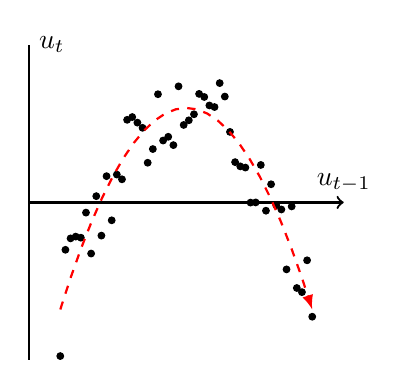
\begin{tikzpicture}[scale=0.20]
				% \draw [step=1, gray, very thin] (0, 0) grid (20, 23);
				\draw [thick, ->] (0, 10) -- (20, 10) node [anchor=south] {$u_{t - 1}$}; 
				\draw [thick, -] (0, 0) -- (0, 20) node [anchor=west] {$u_{t}$}; 
				\draw plot [only marks, mark=*, mark size=6, domain=2:18, samples=50] (\x, {-0.2*(\x - 10)^2 + 13 + 6*rnd}); 
				\draw [thick, dashed, red, -latex] plot [domain=2:18] (\x, {-0.2*(\x - 10)^2 + 16});
			\end{tikzpicture}
		\end{center}
	\end{multicols}
\end{document}
